%!TEX root = ../Manuale.tex
%%--------------------------------------------------------------------------
%% IMPOSTAZIONI
%%--------------------------------------------------------------------------



\chapter{Settings}
On the settings page you can change several aspects:
	\begin{description}

		\item[Connessione all'avvio]
		Allows you to initiate a connection to the server at startup of the device.

		\item[Connessione Server]
		Make the connection with the server.

		\item[Host]
		IP address of the server.

		\item[Porta]
		Port of the server.

		\item[Frequenza di riconnessione]
		Determines the frequency with which it will try to connect to the server when it is not accessible.

		\item[Invio posizione]
		If activated, the device periodically sends its position to the server.

		\item[Frequenza di invio della posizione]
		Determines the frequency with which it will send the device position.

	\end{description}



	\begin{figure}[h!]
		  \centering
		    \centering{%
		      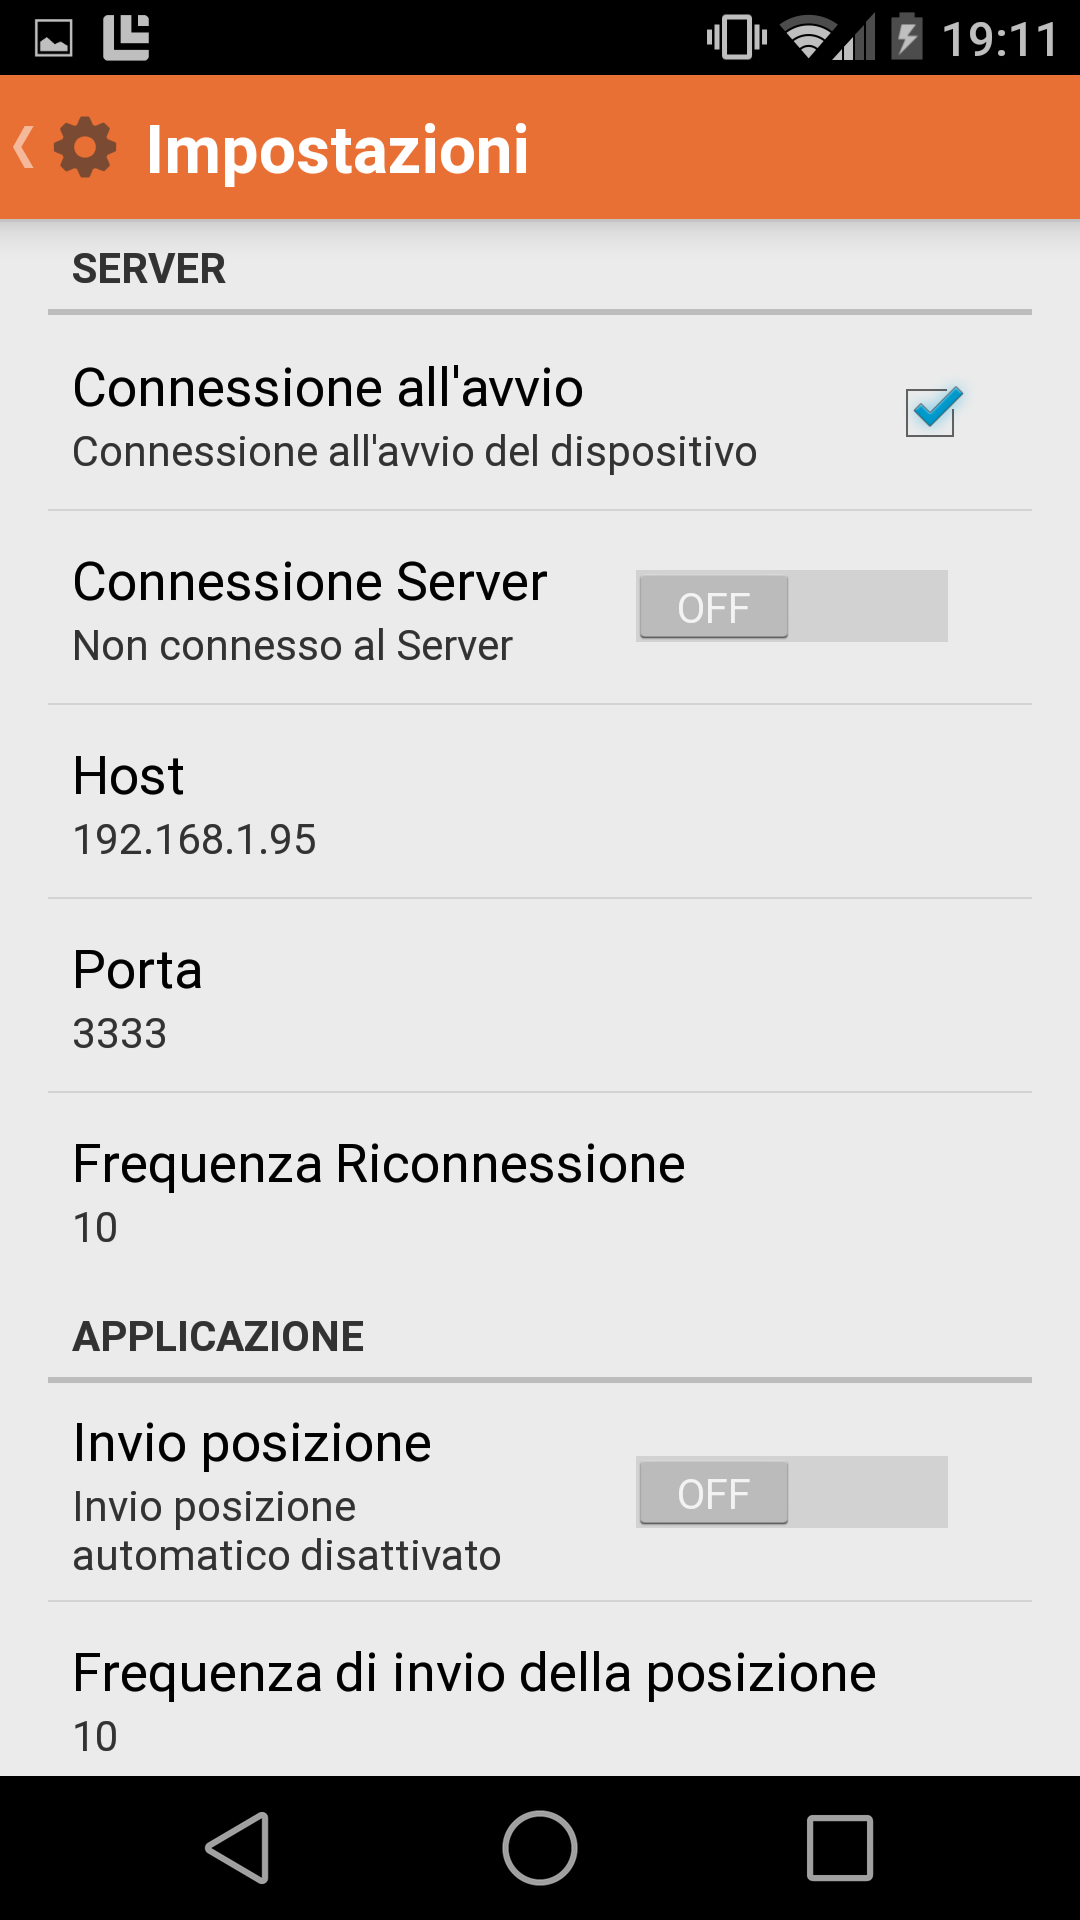
\includegraphics[width=0.7\textwidth]{phone_settings.png}}
		  \caption{Phone - Settings}
	\end{figure}

	\begin{figure}[h!]
		  \centering
		    \centering{%
		      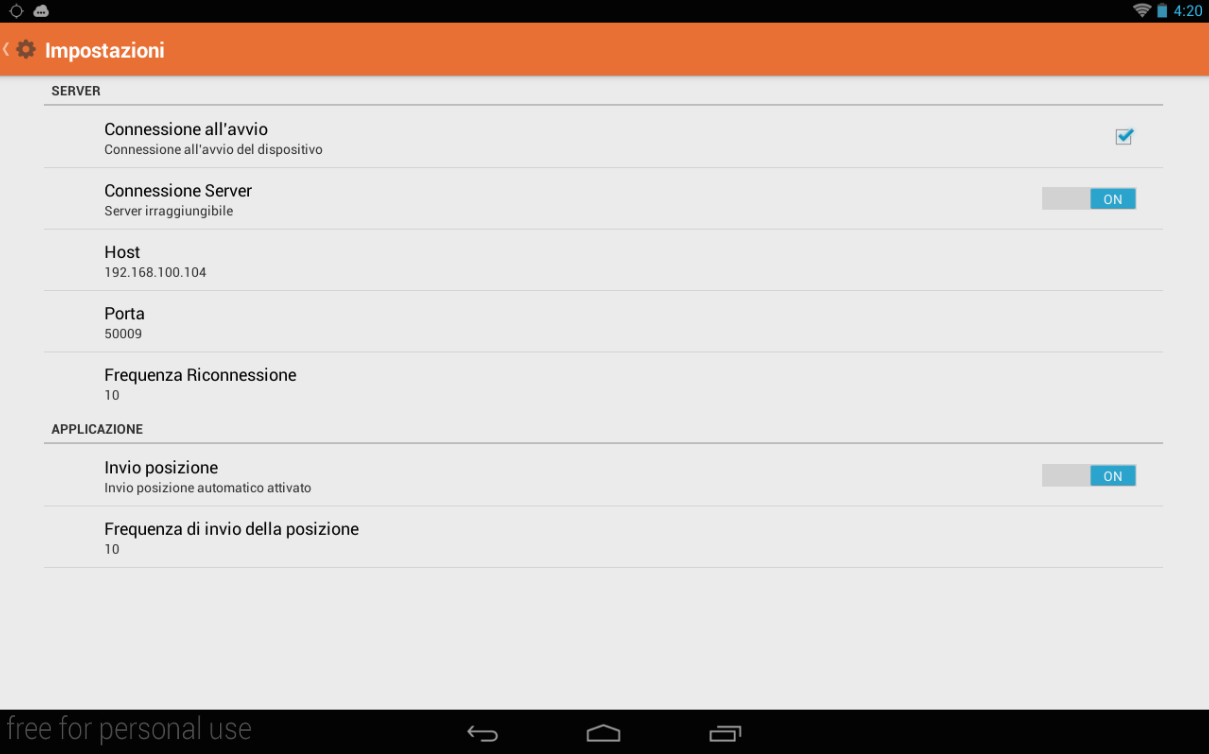
\includegraphics[width=1\textwidth]{tablet_impostazioni.png}}
		  \caption{Tablet - Settings}
	\end{figure}
